%%----------------------------------------------------------------------------------
% DO NOT Change this is the required setting A4 page, 11pt, onside print, book style
%%----------------------------------------------------------------------------------
\documentclass[a4paper,11pt,oneside]{book} 
\usepackage{CS_report} % DO NOT REMOVE THIS LINE. 
%%%%%%%%%%%%%%%%%%%%%%%%%%%%%%%%%%%%%%%%%%%%%%%%%%%%%%%%%%%%%%%%%%%%%%%%%%%%%%%%%%%%


%%%%%%%%%%%%%%%%%%%%%%%%%%%%%%%%%%%%%%%%%%%%%%%%%%%%%%%%%%%%%%%%%%%%%%%%%%%%%%%%%%%%
\begin{document}
    \captionsetup[figure]{margin=1.5cm,font=small,name={Figure},labelsep=colon}
    \captionsetup[table]{margin=1.5cm,font=small,name={Table},labelsep=colon}
    
    \frontmatter
    
    %%%%%%%%%%%%%%%%%%%%%%%%%%%%%%%%%%%%%%%%%%%%%%%%%%%%%%%%%%%%%%%%%%%%%%%%%%%%%%%%
    \begin{titlepage}      
        \begin{center}
            % Comment out UoR logo if not applicable
            
\includegraphics[width=7cm]{figures/UDLogo.png}\\[0.3cm]
            {\LARGE Universidad Distrital Francisco José de Caldas\\[0.3cm]
            Computer Engineering Program\\[0.3cm]
            School of Engineering}\\[2cm]
			
            \linespread{1.0}\huge {
                Workshop No. 1 -- Kaggle Project Analysis: CIBMTR Equity in Post-HCT Survival Predictions
            }
            \linespread{1}~\\[2cm]
            {\Large 
                Sergio Nicolás Mendivelso Martínez -- 20231020227\\
                Sergio Leonardo Moreno Granado -- 20242020091\\
                Juan Manuel Otálora Hernández -- 20242020018\\
                Juan Diego Moreno Ramos - 20242020009\\
            }
            

            {\Large 
                \emph{Professor:} Eng. Carlos Andrés Sierra, M.Sc.}\\[1cm]
            
    		\large A report submitted for Workshop No. 1 in Systems Analysis \& Design\\
            Semester 2025-III 
            \\[0.3cm] 
            \vfill
            
            
            September 2025, Bogotá D.C.
        \end{center}
    \end{titlepage}

     
    % -------------------------------------------------------------------
    % Abstract and Acknowledgement
    % -------------------------------------------------------------------
    
    %Two resources useful for abstract writing.
% Guidance of how to write an abstract/summary provided by Nature: https://cbs.umn.edu/sites/cbs.umn.edu/files/public/downloads/Annotated_Nature_abstract.pdf %https://writingcenter.gmu.edu/guides/writing-an-abstract
\chapter*{\center \Large  Abstract}
%%%%%%%%%%%%%%%%%%%%%%%%%%%%%%%%%%%
% Replace all text with your text
%%%%%%%%%%%%%%%%%%%%%%%%%%%%%%%%%%%

This workshop presents a comprehensive systems analysis of the CIBMTR (Center for International Blood and Marrow Transplant Research) Kaggle competition focused on equity in post-hematopoietic cell transplant (HCT) survival predictions. The competition challenges participants to develop machine learning models that accurately predict survival outcomes following allogeneic hematopoietic cell transplantation while ensuring fairness across different racial and socioeconomic groups.

\vspace{0.3cm}

Our analysis examines the complexity of the medical system surrounding HCT procedures, identifies key variables affecting patient outcomes, and evaluates the dual requirements of accuracy and equity in predictive modeling. The study reveals the intricate relationships between clinical, genetic, and demographic factors that influence post-transplant survival, highlighting the system's sensitivity to small parameter variations and the presence of chaotic behavior in medical outcomes.

\vspace{0.3cm}

Key findings include the identification of critical sensitivity parameters such as patient age, disease risk indices, genetic compatibility scores, and comorbidities. The analysis emphasizes the importance of the stratified C-index evaluation metric, which ensures model performance is consistent across ethnic subgroups. This work contributes to understanding how systems thinking can be applied to improve both the accuracy and fairness of medical prediction models, with direct implications for personalized medicine and transplant care.

\vspace{0.3cm}

The integration of recent advances in machine learning approaches for hematopoietic stem cell research demonstrates the evolving landscape of predictive modeling in healthcare. Our recommendations include implementing ensemble methods, maintaining demographic balance in cross-validation strategies, and incorporating domain expertise in feature engineering to address the inherent complexity and randomness in biological systems.

\vspace{0.3cm}

\textbf{Keywords:} Hematopoietic Cell Transplantation, Machine Learning, Healthcare Equity, Systems Analysis, Survival Prediction, Medical Informatics, Artificial Intelligence, Predictive Modeling % Insert a brief abstract summarizing the analysis, objectives, and key findings.
    % -------------------------------------------------------------------
	% Acknowledgement
	% -------------------------------------------------------------------
    
    % -------------------------------------------------------------------
    % Contents, list of figures, list of tables
    % -------------------------------------------------------------------
    
    \tableofcontents
    \listoffigures
    %\listoftables
    %\input{glossaries} % List abbreviations: e.g., HCT: Hematopoietic Cell Transplantation, EFS: Event-Free Survival, C-index: Concordance Index.

    %%%%%%%%%%%%%%%%%%%%%%%%%%%%%%%%%%%%%%%%%%%%%%%%%%%%%%%%%%%%%%%%%%%%%%%
    %%                                                                    %%  
    %%  Main chapters and sections of your project                        %%  
    %%  Everything from here on needs updates in your own words and works %%
    %%                                                                    %%
    %%%%%%%%%%%%%%%%%%%%%%%%%%%%%%%%%%%%%%%%%%%%%%%%%%%%%%%%%%%%%%%%%%%%%%%%
    \mainmatter
    
    \chapter{Introduction and System Analysis}

\section{Overview}

The ``CIBMTR – Equity in Post-HCT Survival Predictions'' competition has as its primary objective the development of models that accurately predict survival outcomes after allogeneic hematopoietic cell transplantation (HCT) \cite{kaggle_competition}. What distinguishes this competition is its dual approach: predictions must not only be accurate but also equitable, addressing existing disparities by ensuring that models do not disadvantage patients based on their demographic or socioeconomic background.

\vspace{0.3cm}

The provided dataset contains clinical, genetic, and demographic information for each patient. Relevant variables include age, ethnicity, disease risk indices, genetic compatibility metrics, and detailed medical histories \cite{cibmtr_datasets}. By leveraging this multifaceted data, the goal is to promote innovations in predictive modeling that can directly inform and improve personalized medicine and transplant care.

\vspace{0.3cm}

The main competition rules are as follows: Data use is strictly limited to the datasets provided within the competition framework; external data is not permitted unless explicitly authorized. Additionally, participants must meet equity criteria, as solutions will be evaluated not only for their overall accuracy but also for their equitable performance across different patient groups \cite{kaggle_competition}.

\vspace{0.3cm}

\section{Objectives}

This workshop aims to achieve the following interconnected objectives:
\begin{itemize}
    \item Understand the structure of the competition's system
    \item Learn more about the medical context to apply new ideas as accurately as possible
    \item Identify the system's elements, relationships, and boundaries
    \item Check the sensitivity and complexity of the problem
    \item Analyze the evaluation metric
    \item Propose recommendations to improve the accuracy and fairness of the models
\end{itemize}

\section{Medical Background}

\subsection{Allogeneic Hematopoietic Cell Transplantation}

Allogeneic Hematopoietic Cell Transplantation (HCT) is a medical procedure where a patient receives healthy blood stem cells from a compatible donor \cite{uptodate_hct}. These new cells replace the patient's damaged or sick bone marrow and help rebuild a working blood and immune system. Recent advances in transplantation have significantly improved patient survival over time, though high morbidity and mortality risks remain critical challenges \cite{astct_simplification}.

The term allogeneic means the cells come from another person (a relative or someone unrelated). Although stem cells can be collected in different ways, bone marrow remains a primary source for transplantation \cite{aacr_historical}.

This procedure is mainly used to treat serious blood and immune system diseases, such as:
\begin{itemize}
    \item Acute and chronic leukemias \cite{ash_transplant_all}
    \item Lymphomas
    \item Multiple myeloma
    \item Severe aplastic anemia
    \item Immune disorders \cite{biorxiv_autoimmune}
\end{itemize}

The goal is to replace faulty or harmful cells with stem cells that can create healthy new blood cells like red blood cells, white blood cells (T and B lymphocytes), and platelets \cite{uptodate_hct}.

\subsection{The Transplantation Process}

The HCT process involves several critical stages \cite{uptodate_hct}:

\begin{enumerate}
    \item \textbf{Donor selection:} A genetic compatibility test (HLA typing) is performed. The better the match, the lower the risk of rejection. This is where prediction models from the competition become relevant.
    
    \item \textbf{Patient preparation:} Before the transplant, the patient receives chemotherapy and/or radiation to:
    \begin{itemize}
        \item Destroy diseased cells
        \item Suppress the immune system to prevent rejection
    \end{itemize}
    
    \item \textbf{Stem cell infusion:} The transplant is not a surgical procedure. Stem cells are administered through an IV, similar to a blood transfusion.
    
    \item \textbf{Engraftment:} The donor's stem cells travel to the patient's bone marrow and begin producing new blood cells. Recent studies have shown that robust and polyclonal engraftment occurs across different age groups, though with distinct differences in cellular diversity \cite{stmcls_clonality}.
    
    \item \textbf{Follow-up:} Patients require close monitoring to detect and manage complications.
\end{enumerate}

\subsection{Risks and Complexity}

Because the transplant uses cells from another person, there is a risk that the patient's body may recognize them as foreign. Laboratory tests are conducted to reduce the likelihood of rejection or immune reactions \cite{uptodate_gvhd}.

Possible complications include:
\begin{itemize}
    \item \textbf{Graft-versus-host disease (GVHD):} The donor's immune cells may attack the patient's tissues \cite{uptodate_gvhd, ash_chronic_gvhd}
    \item \textbf{Infections}
    \item \textbf{Graft failure:} The new cells fail to engraft or function properly
    \item \textbf{Social and geographic factors:} These can affect access to care, treatment follow-up, and overall outcomes \cite{mdpi_cancers}
\end{itemize}

\subsection{Importance of Survival Prediction}

Allogeneic transplants are high-risk and expensive procedures \cite{astct_simplification}. Accurate survival prediction:
\begin{itemize}
    \item Helps physicians make better decisions about transplant candidacy
    \item Enables more personalized treatment and care protocols
    \item Improves utilization of healthcare resources
    \item Reduces health inequalities, as current models often favor certain population groups \cite{jama_ai_medicine}
\end{itemize}

\section{System Analysis}

\subsection{Input Data Sources and Characteristics}

The predictive system incorporates comprehensive data sources spanning clinical, transplant-specific, demographic, and temporal dimensions:

\subsubsection{Disease and Clinical Characteristics}
\begin{itemize}
    \item Disease characteristics: Type of hematological malignancy, disease stage at transplant, remission status
    \item Pre-transplant comorbidity indices: Existing health conditions that affect transplant outcomes
    \item Previous treatment history: Chemotherapy cycles, radiation exposure, prior transplants
    \item Laboratory values: Blood counts, organ function markers, inflammatory markers
    \item Karnofsky/Lansky performance scores: Functional status indicators
\end{itemize}

\subsubsection{Transplant-Specific Inputs}
\begin{itemize}
    \item Donor type: Matched related, matched unrelated, haploidentical, cord blood
    \item HLA matching degree: Level of compatibility between donor and recipient
    \item Stem cell source: Bone marrow, peripheral blood, umbilical cord
    \item Conditioning regimen intensity: Myeloablative, reduced intensity, non-myeloablative
    \item Graft-versus-host disease prophylaxis protocol
\end{itemize}

\subsubsection{Demographic and Socioeconomic Inputs}
\begin{itemize}
    \item Age at transplant (continuous variable)
    \item Sex/gender (categorical)
    \item Race/ethnicity (categorical, critical for equity analysis)
    \item Geographic location (affects access to care)
    \item Insurance status (impacts follow-up care quality)
\end{itemize}

\subsubsection{Temporal Inputs}
\begin{itemize}
    \item Year of transplant (captures medical advances over time)
    \item Time from diagnosis to transplant (affects disease progression)
    \item Follow-up duration markers
\end{itemize}

\subsection{System Architecture and Modules}

The predictive system employs a sophisticated modular architecture designed to ensure both accuracy and equity in survival predictions:

\subsubsection{Data Preprocessing Module}
This module handles initial data preparation through multiple stages:
\begin{itemize}
    \item Feature engineering: Creating interaction terms between clinical and demographic variables, calculating risk scores from raw measurements, generating time-dependent features
    \item Data standardization and normalization while preserving demographic-related variations that might mask inequities
    \item Handling missing data and outliers with equity-aware imputation methods
\end{itemize}

\subsubsection{Equity Analysis Module}
This component specifically addresses fairness in the model:
\begin{itemize}
    \item Stratified analysis across demographic groups to identify potential biases
    \item Bias detection algorithms measuring disparities in data quality, feature availability, and baseline outcome rates
    \item Fairness-aware preprocessing techniques, such as reweighting samples to balance representation across demographic groups while preserving clinical validity
\end{itemize}

\subsubsection{Feature Selection and Importance Module}
This system component determines which variables contribute most to survival predictions:
\begin{itemize}
    \item Multiple selection strategies: Clinical domain knowledge integration, statistical significance testing, machine learning-based feature importance rankings
    \item Ensuring predictive features are available equitably across all patient populations
    \item Avoiding features that might be systematically missing for certain demographic groups
\end{itemize}

\subsubsection{Predictive Modeling Core}
The central prediction engine employs an ensemble approach:
\begin{itemize}
    \item Survival analysis models: Cox proportional hazards and accelerated failure time models for time-to-event predictions
    \item Machine learning algorithms: Gradient boosting machines and random forests for complex pattern recognition
    \item Deep learning architectures for capturing non-linear relationships
    \item Cross-validation specifically designed for survival data with demographic stratification
\end{itemize}

\subsubsection{Fairness Calibration Module}
This post-processing component adjusts model predictions for equitable performance:
\begin{itemize}
    \item Calibration techniques maintaining similar prediction accuracy across different patient populations
    \item Threshold optimization considering fairness metrics alongside traditional performance measures
    \item Disparity impact assessment to quantify and minimize prediction inequities
\end{itemize}

\subsubsection{Uncertainty Quantification Module}
This component provides confidence intervals and prediction uncertainties:
\begin{itemize}
    \item Prediction intervals using techniques appropriate for survival analysis
    \item Risk stratification with associated uncertainty bounds
    \item Identification of cases where predictions might be less reliable due to data limitations
\end{itemize}

\subsection{System Outputs}

The system generates comprehensive outputs for clinical decision support and equity monitoring:

\subsubsection{Primary Output}
\begin{itemize}
    \item Survival Probability Predictions: Time-dependent survival probabilities at key clinical milestones (100 days, 1 year, 2 years, 5 years post-transplant)
    \item Risk Stratification Categories: Patient classification into risk groups (low, intermediate, high) with associated survival curves
\end{itemize}

\subsubsection{Secondary Outputs}
\begin{itemize}
    \item Equity Metrics Dashboard: Comprehensive fairness assessments including demographic parity measures showing prediction consistency across groups
    \item Clinical Decision Support Outputs: Individualized risk factors highlighting important predictors, comparative analysis showing patient risk profiles, treatment modification suggestions based on modifiable risk factors
    \item Model Interpretability Outputs: Feature importance rankings, partial dependence plots, SHAP values providing detailed explanations for individual predictions
    \item Quality Assurance Outputs: Model performance metrics, calibration plots, data quality reports identifying input data issues
    \item Research and Monitoring Outputs: Aggregate statistics for clinical research, temporal trend analyses, center-specific performance metrics for transplant program evaluation
\end{itemize}

\section{Complexity and Sensitivity Analysis}

\subsection{Complexity in Post-HCT Survival Modeling}

The challenge of predicting survival outcomes after hematopoietic cell transplantation (HCT) lies fundamentally in the system's complexity \cite{astct_simplification}. Multiple interconnected clinical, genetic, and demographic factors influence patient survival, from age, disease stage, and comorbidities to donor compatibility and care protocols. The interaction of these variables forms a nonlinear, high-dimensional system where unexpected effects can arise from subtle parameter changes \cite{frontiers_ai_hct}.

\vspace{0.3cm}

Furthermore, feedback effects, such as immune responses, transplant complications, or secondary interventions, can introduce new layers of complexity, making simple models insufficient to capture the true patient trajectory \cite{stmcls_clonality}.

\subsection{Sensitivity Analysis}

Small variations in input variables can cause significant differences in survival predictions. For example, changing a patient's age or disease risk index value can substantially modify the survival estimate, relocating the patient to another risk group or altering their prognosis \cite{mdpi_cancers}. Similarly, the presence or absence of certain comorbidities (such as renal failure or previous infections) can generate major changes in the final model outcome.

\vspace{0.3cm}

A technique used to measure this complexity is subgroup analysis, whereby dividing the sample into subgroups (by age, gender) and examining how predictions change can analyze the system's sensitivity to these changes.

\textbf{Sensitive parameters include:}
\begin{itemize}
    \item \textbf{Age:} An increase of only one year can move a patient from a low to high-risk category \cite{stmcls_clonality}
    \item \textbf{Disease risk index:} Small changes in the score can alter prognosis or eligibility for specific treatments
    \item \textbf{Genetic compatibility:} Minimal differences can affect transplant rejection rates and survival
    \item \textbf{Severe comorbidities:} Their presence or absence can double or drastically reduce projected survival
\end{itemize}

\subsection{Chaos and Randomness in Post-HCT Survival Prediction}

Medical outcomes following allogeneic hematopoietic cell transplantation (HCT) are intrinsically unpredictable and complex, with many processes exhibiting characteristics of chaos and randomness \cite{frontiers_ai_hct}. Chaos theory, which describes how small variations in initial conditions can lead to vastly different outcomes, is highly relevant for survival modeling in this context. Even small inaccuracies or variations in clinical measurements, such as patient age, genetic compatibility, or comorbidities, can dramatically change survival predictions.

\vspace{0.3cm}

This sensitivity is sometimes known as the ``butterfly effect'' in nonlinear systems. Randomness also plays a key role. Patient data contain elements of stochasticity arising from biological diversity, incomplete records, and unknown confounding factors \cite{biorxiv_autoimmune}. For example, two patients with apparently identical risk factors may experience completely different outcomes after transplantation due to hidden genetic or environmental variables.

\vspace{0.3cm}

Therefore, the proposed model must be robust against noise, outliers, and missing data, as these introduce additional layers of unpredictability in survival outcomes. Furthermore, feedback loops and nonlinearities, such as immune responses or treatment complications, can give rise to emergent behaviors that are difficult to predict using traditional linear models \cite{frontiers_immunology}. These dynamic interactions illustrate how system evolution cannot be fully explained or predicted by examining its individual parts in isolation. Even the most advanced predictive models may struggle to capture all aspects of post-HCT survival, highlighting the ever-present influence of chaos and randomness in personalized medicine.

\section{Evaluation and Metrics}

\subsection{The C-Index Metric}

The C-Index is a metric used to evaluate a survival model's ability to correctly order risk among pairs of patients \cite{kaggle_competition}. In the Kaggle competition on post-HCT survival, a ``stratified'' version is used, meaning the C-index is calculated within each racial group of patients and then these results are averaged with dispersion adjustment. This stratified C-Index dictates that our model must be not only accurate overall but consistent and fair across all ethnic subgroups present in the dataset.

\subsection{Importance of Equity in Medical Predictions}

Equity in medical predictions is fundamental because it ensures that all patients, regardless of their race, gender, socioeconomic status, or other factors, receive fair and accurate care \cite{jama_ai_medicine}. When predictive models do not consider equity, they can perpetuate existing inequalities in the health system.

\section{Visual Representation}

\begin{figure}[htbp]
    \centering
    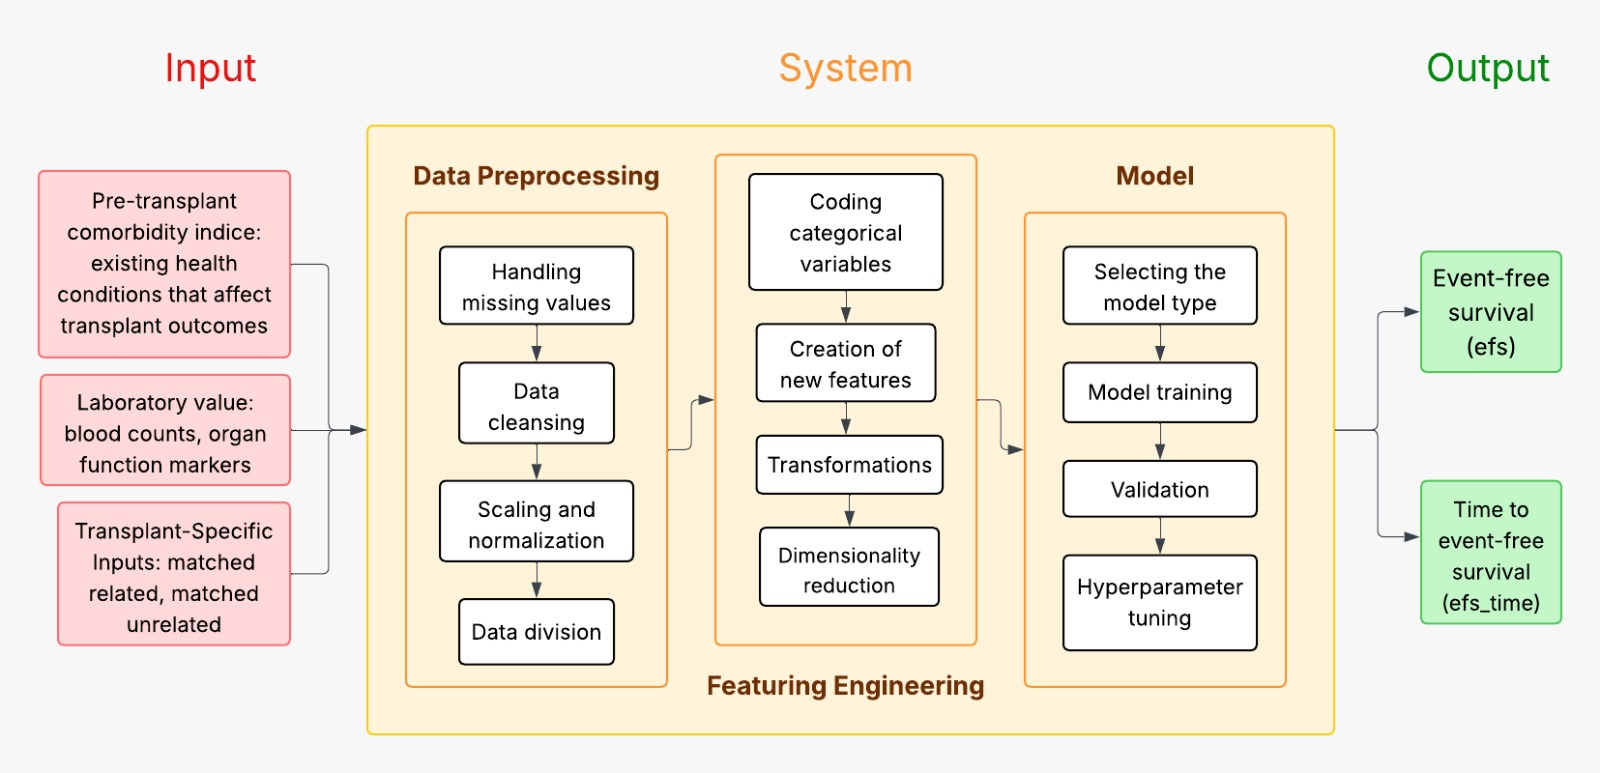
\includegraphics[width=1\textwidth]{figures/SystemDiagram.jpg}
    \caption{Diagram illustrating the modular pipeline of the predictive system. The diagram shows the flow from input data sources through preprocessing, equity analysis, feature selection, predictive modeling, fairness calibration, and uncertainty quantification modules, culminating in the output of survival predictions and equity metrics.}
    \label{fig:system_architecture}
\end{figure}

\section{Conclusions}

\subsection{Key Findings Summary}

This analysis reveals several critical aspects of the CIBMTR competition system:

\begin{itemize}
    \item The complexity of post-HCT survival prediction stems from multiple interacting clinical, demographic, and transplant-specific factors
    \item The modular system architecture enables both accurate predictions and equitable performance across demographic groups
    \item Small parameter variations can significantly impact predictions, requiring robust sensitivity analysis
    \item The stratified C-index metric ensures equitable model performance while maintaining clinical accuracy
    \item System sensitivity requires sophisticated modeling approaches with built-in fairness calibration
\end{itemize}

\subsection{System Strengths and Weaknesses}

\textbf{Strengths:}

\begin{itemize}
    \item Comprehensive multi-modular architecture addressing both accuracy and equity \cite{kaggle_competition}
    \item Integrated fairness calibration throughout the prediction pipeline
    \item Real-world medical application with high impact potential \cite{astct_simplification}
    \item Sophisticated handling of clinical complexity through ensemble modeling approaches \cite{frontiers_ai_hct}
    \item Comprehensive output system supporting clinical decision-making and equity monitoring
\end{itemize}

\textbf{Weaknesses:}

\begin{itemize}
    \item High system complexity requires substantial computational resources
    \item Inherent randomness and chaos in biological systems \cite{biorxiv_autoimmune}
    \item Potential for hidden confounding variables not captured in current data sources
    \item Dependence on data quality and completeness across all demographic groups
    \item Challenges in generalizing across different healthcare systems and populations
\end{itemize}

\subsection{Recommendations}

To improve accuracy and equity in predictions:

\begin{itemize}
    \item Implement advanced ensemble methods to handle system complexity while maintaining interpretability \cite{frontiers_ai_hct}
    \item Develop cross-validation strategies that maintain demographic balance across all folds
    \item Create robust preprocessing techniques specifically designed for clinical missing data patterns
    \item Incorporate domain expertise in feature engineering to ensure clinical relevance
    \item Apply fairness-aware regularization techniques to prevent overfitting to majority groups
    \item Consider temporal dynamics and evolving medical practices in patient outcomes \cite{stmcls_clonality}
    \item Enhance uncertainty quantification to support clinical decision-making under uncertainty
\end{itemize}

\subsection{Clinical and Healthcare System Implications}

This work has significant implications for:

\begin{itemize}
    \item Enhanced clinical decision-making in transplant medicine through personalized risk assessment \cite{astct_simplification}
    \item More equitable allocation of medical resources based on accurate and fair predictions
    \item Advancement of personalized medicine approaches through comprehensive risk profiling \cite{biorxiv_autoimmune}
    \item Reduction of healthcare disparities through systematic bias detection and mitigation \cite{jama_ai_medicine}
    \item Development of fair AI systems in healthcare that can be trusted across diverse populations
    \item Improved patient outcomes through better risk stratification and targeted interventions
    \item Quality improvement in transplant programs through comprehensive monitoring and evaluation outputs
\end{itemize} % Paste Introduction content: Brief context, importance, objectives (Comprender la estructura..., etc.).
    
    % -------------------------------------------------------------------
    % Bibliography/References
    % -------------------------------------------------------------------
    \bibliography{references}  % Add entries for sources: academic papers, official documents, web pages.
    
\end{document}